\let\negmedspace\undefined
\let\negthickspace\undefined
\documentclass[journal,12pt,twocolumn]{IEEEtran}

\usepackage{csquotes}
\usepackage{comment}
\usepackage{enumerate}
\usepackage{amsmath,amssymb,amsthm}
\usepackage{graphicx}
\let\vec\mathbf
\newcommand{\myvec}[1]{\ensuremath{\begin{pmatrix}#1\end{pmatrix}}}
\providecommand{\brak}[1]{\ensuremath{\left(#1\right)}}
\providecommand{\pr}[1]{\ensuremath{\Pr\left(#1\right)}}


     \title{Assignment 1}
     \author{AKKASANI YAGNESH REDDY \\
     cs21btech11003 \\
     ICSE 2019 12th 16a}
     

\begin{document}

     \maketitle
\textbf{Question:} If $\vec{a}=i-2j+3k$,$\vec{b}=2i+3j-5k$. prove that $\vec{a}$ and $\vec{a}\times\vec{b}$ are perpendicular.\\
    
    \textbf{Solution:}Given vectors
    \begin{align}
        \vec{a}=\myvec{1\\-2\\3} \\
        \vec{b}=\myvec{2\\3\\-5}
    \end{align}
    
    Cross product between vectors is defined by,If
    \begin{align}
        \vec{a}=\myvec{a_{1}\\a_{2}\\a_{3}}\\
        \vec{b}=\myvec{b_{1}\\b_{2}\\b_{3}}
    \end{align}
        Then,
    \begin{align}
            \vec{a}\times\vec{b}=\myvec{a_{2}b_{3}-a_{3}b_{2}\\a_{3}b_{1}-a_{1}b_{3}\\a_{1}b_{2}-a_{2}b_{1}}
    \end{align}
      
      By following the definition and substituting values we get
      
      \begin{align}
          \vec{a}\times\vec{b}&=\myvec{(-2)(-5)-(3)(3)\\(3)(2)-(-5)(1)\\(1)(3)-(-2)(2)}\\ 
         \Rightarrow  \vec{a}\times\vec{b}&=\myvec{1\\11\\7}
           \end{align}
         $\vec{a}$ and  $\vec{a}\times\vec{b}$ are perpendicular if dot product between them is $0$.  
    Dot product between two vector $\vec{a}$ and $\vec{b}$ is, If
    \begin{align}
        \vec{a}=\myvec{a_{1}\\a_{2}\\a_{3}}\\
        \vec{b}=\myvec{b_{1}\\b_{2}\\b_{3}}
    \end{align}
    Then,
    \begin{align}
      \vec{a}.\vec{b}=a_{1}b_{1}+a_{2}b_{2}+a_{3}b_{3}
    \end{align}
          Substituting values,
          \begin{align}
              \vec{a}. (\vec{a}\times\vec{b})&=(1)(2)+(-2)(3)+(3)(-5)\\
              \Rightarrow\vec{a}. (\vec{a}\times\vec{b})&=0
          \end{align}
          
          
          Hence both $\vec{a}$ and $\vec{a}\times\vec{b}$ are perpendicular to each other.
          \begin{figure}[h!]
              \centering
              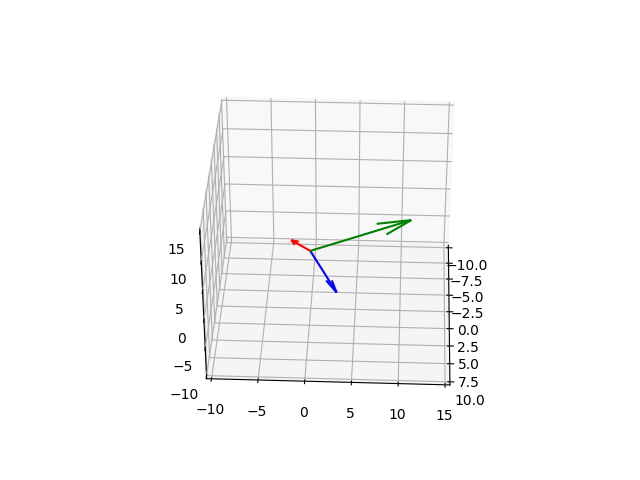
\includegraphics{A2python.png}
              \caption{Python generated figure}
              \label{fig:my_label}
          \end{figure}
          
\end{document}